\begin{frame}{Recall: MultiLayer Perceptron (MLP)}
\centering
        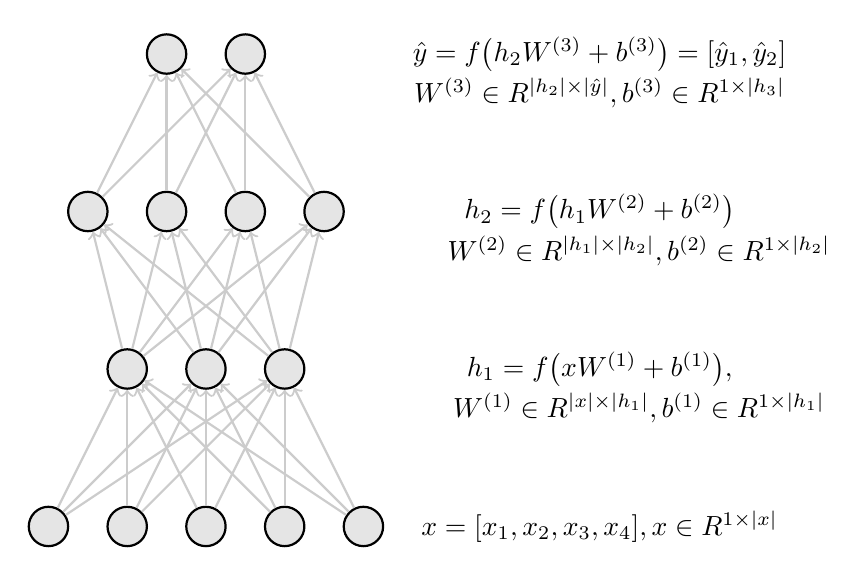
\begin{tikzpicture}
        \tikzset{node/.style={draw,circle, minimum width=0.5cm, fill=gray!20, thick}}
        \tikzset{edge/.style={draw, thick, black!20, ->}}
        
            \node(x1) at (0, 0) [node] {};
            \node(x2) at (1, 0) [node] {};
            \node(x3) at (2, 0) [node] {};
            \node(x4) at (3, 0) [node] {};
            \node(x5) at (4, 0) [node] {};
            
            \node(x_label) at (7,0.0) {$\bm{x} = [x_1, x_2, x_3, x_4 ], \bm{x} \in \mathbb{R}^{1 \times |\bm{x}|}$};
            
            \node(h11) at (1, 2) [node] {};
            \node(h12) at (2, 2) [node] {};
            \node(h13) at (3, 2) [node] {};
            
            \node(h1_label) at (7,2) {$\bm{h_1}= f \big( \bm{x}\bm{W^{(1)}} + \bm{b^{(1)}} \big), $};
            \node(h1_dim) at (7.5,1.5) {$\bm{W^{(1)}} \in \mathbb{R}^{|\bm{x}| \times |\bm{h_1}|}, \bm{b^{(1)}} \in \mathbb{R}^{1 \times |\bm{h_1}|}  $};
                
            \node(h21) at (0.5, 4) [node] {};
            \node(h22) at (1.5, 4) [node] {};
            \node(h23) at (2.5, 4) [node] {};
            \node(h24) at (3.5, 4) [node] {};
            
            \node(h2_label) at (7,4) {$\bm{h_2}= f \big( \bm{h_1} \bm{W^{(2)}} + \bm{b^{(2)}} \big)$};
            \node(h2_dim) at (7.5,3.5) {$ \bm{W^{(2)}} \in \mathbb{R}^{|\bm{h_1}| \times |\bm{h_2}|}, \bm{b^{(2)}} \in \mathbb{R}^{1 \times |\bm{h_2}|} $};
            
            \node(y1) at (1.5, 6) [node] {};
            \node(y2) at (2.5, 6) [node] {};
            
            
            \node(h2_label) at (7,6) {$\bm{\hat{y}}= f \big( \bm{h_2}\bm{W^{(3)}} + \bm{b^{(3)}} \big) = [\hat{y}_1, \hat{y}_2] $};
            \node(h2_dim) at (7,5.5) { $\bm{W^{(3)}} \in \mathbb{R}^{|\bm{h_2}| \times |\bm{\hat{y}}|}, \bm{b^{(3)}} \in \mathbb{R}^{1 \times |\bm{h_3}|} $};
            
            
            
            \draw[edge] (x1) -- (h11);
            \draw[edge] (x2) -- (h11);
            \draw[edge] (x3) -- (h11);
            \draw[edge] (x4) -- (h11);
            \draw[edge] (x5) -- (h11);
            

            \draw[edge] (x1) -- (h12);
            \draw[edge] (x2) -- (h12);
            \draw[edge] (x3) -- (h12);
            \draw[edge] (x4) -- (h12);
            \draw[edge] (x5) -- (h12);
            
            \draw[edge] (x1) -- (h13);
            \draw[edge] (x2) -- (h13);
            \draw[edge] (x3) -- (h13);
            \draw[edge] (x4) -- (h13);
            \draw[edge] (x5) -- (h13);
            
            \draw[edge] (h11) -- (h21);
            \draw[edge] (h11) -- (h22);
            \draw[edge] (h11) -- (h23);
            \draw[edge] (h11) -- (h24);
            
            
            \draw[edge] (h12) -- (h21);
            \draw[edge] (h12) -- (h22);
            \draw[edge] (h12) -- (h23);
            \draw[edge] (h12) -- (h24);
            
            \draw[edge] (h13) -- (h21);
            \draw[edge] (h13) -- (h22);
            \draw[edge] (h13) -- (h23);
            \draw[edge] (h13) -- (h24);
            
            \draw[edge] (h21) -- (y1);
            \draw[edge] (h22) -- (y1);
            \draw[edge] (h23) -- (y1);
            \draw[edge] (h24) -- (y1);

            \draw[edge] (h21) -- (y2);
            \draw[edge] (h22) -- (y2);
            \draw[edge] (h23) -- (y2);
            \draw[edge] (h24) -- (y2);


        \end{tikzpicture}
    

\end{frame}
\begin{frame}{Recall: Feedforward}
\centering
        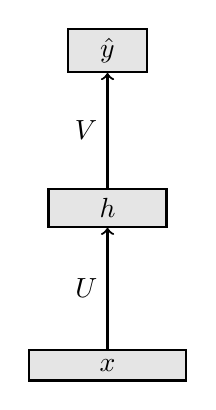
\begin{tikzpicture}
            \tikzset{layer/.style={draw,rectangle, fill=gray!20, thick}}
            \tikzset{edge/.style={->, thick}}
        
            \node(x) at (0,0) [layer, minimum width=2cm] {$\bm{x}$};
            \node(h) at (0,2) [layer, minimum width=1.5cm] {$\bm{h}$};
            \node(y_hat) at (0,4) [layer, minimum width=1cm] {$\bm{\hat{y}}$};
        
        
            \draw[edge](x) --node[left]{$\bm{U}$} (h);
            \draw[edge](h) -- node[left]{$\bm{V}$} (y_hat);
        
        
        \end{tikzpicture}
    

\end{frame}
\begin{frame}{Motivation}
    \begin{itemize}
        \item Text is a \textbf{sequence} of symbols.
        \item Symbols show characters, words etc.
        \item input = ``a persian cat on the mat .'' $\longrightarrow$ \\ input = $\big( x_1=$a, $x_2=$persian, $x_3=$cat, $x_4=$sat, $x_5=$on, $x_6=$the, $x_7=$mat$ \big) $ 
        \item As such symbols are related to each other in text, so should symbols' representations. 
        \item How can we relate representations of symbols to each other? 
    \end{itemize}
\end{frame}
\begin{frame}{Recurrent}
\centering
        \begin{tikzpicture}
            \tikzset{layer/.style={draw,rectangle, fill=gray!20, thick}}
            \tikzset{edge/.style={->, thick}}
        
            \node(x1) at (0,0) [layer, minimum width=2cm] {$\bm{x_1}$};
            \node(h1) at (0,2) [layer, minimum width=1.5cm] {$\bm{h_1}$};
            \node(y1_hat) at (0,4) [layer, minimum width=1cm] {$\bm{\hat{y_1}}$};
            \draw[edge](x1) -- node[left]{$\bm{U}$} (h1);
            \draw[edge](h1) -- node[left]{$\bm{V}$} (y1_hat);
        

            \node(x2) at (3,0) [layer, minimum width=2cm] {$\bm{x_2}$};
            \node(h2) at (3,2) [layer, minimum width=1.5cm] {$\bm{h_2}$};
            \node(y2_hat) at (3,4) [layer, minimum width=1cm] {$\bm{\hat{y_2}}$};
            \draw[edge](x2) -- node[left]{$\bm{U}$} (h2);
            \draw[edge](h2) -- node[left]{$\bm{V}$} (y2_hat);
        
            \node(x3) at (6,0) [layer, minimum width=2cm] {$\bm{x_3}$};
            \node(h3) at (6,2) [layer, minimum width=1.5cm] {$\bm{h_3}$};
            \node(y3_hat) at (6,4) [layer, minimum width=1cm] {$\bm{\hat{y_3}}$};
            \draw[edge](x3) -- node[left]{$\bm{U}$} (h3);
            \draw[edge](h3) -- node[left]{$\bm{V}$} (y3_hat);
        
            \node(etc) at (8,2) [] {...};
            
            \draw[edge, myblue] (h1) -- node[above]{$\bm{W}$} (h2);
            \draw[edge,myblue] (h2) -- node[above]{$\bm{W}$} (h3);
            \draw[edge,myblue] (h3) -- node[above]{$\bm{W}$} (etc);
        
        \end{tikzpicture}
\end{frame}
\begin{frame}{Recurrent}
\centering
        \begin{tikzpicture}
            \tikzset{layer/.style={draw,rectangle, fill=gray!20, thick}}
            \tikzset{edge/.style={->, thick}}
        
           
            \node(xt) at (0,0) [layer, minimum width=2cm] {$\bm{x_t}$};
            \node(ht) at (0,2) [layer, minimum width=1.5cm] {$\bm{h_t}$};
            \node(yt_hat) at (0,4) [layer, minimum width=1cm] {$\bm{\hat{y_t}}$};
            \draw[edge](xt) -- node[left]{$\bm{U}$} (ht);
            \draw[edge](ht) -- node[left]{$\bm{V}$} (yt_hat);
            
            \draw[edge, myblue] (0,2.7) -- (-2,2.7);
            \draw[edge, myblue] (-2,2.7) -- node[left]{$\bm{W}$} (-2,1.3);
            \draw[edge, myblue] (-2,1.3) --  (-0.2,1.3); 
            \draw[edge, myblue] (-0.2,1.3) --  (-0.2,1.7);
        \end{tikzpicture}
\end{frame}
\begin{frame}{Recurrent}
    \begin{itemize}
        \item input = a sequence of vectors = $[\bm{x_1},\bm{x_2},\bm{x_3},...,\bm{x_n}]$, $\bm{x_t} \in \mathbb{R}^{1\times |x|}$
        
        \item 
        \begin{equation*}
            \bm{h_t} =  f \big( \bm{x_t}U + \textcolor{myblue}{\bm{h_{t-1}}W} + \bm{b_h}  \big)
        \end{equation*}
        \begin{itemize}
            \item $\bm{U} \in \mathbb{R}^{|x|\times |h|} $, $|h|$ is the dimensionality of hidden states
            \item $\bm{W} \in \mathbb{R}^{|h|\times |h|} $
            \item $\bm{b_h} \in \mathbb{R}^{1\times |h|} $
        \end{itemize}
    \item 
        \begin{equation*}
            \bm{\hat{y}_t} =  g \big( \bm{h_t}V + \bm{b_{\hat{y}}}  \big)
        \end{equation*}
        
                \begin{itemize}
            \item $\bm{V} \in \mathbb{R}^{|h|\times |\hat{y}|} $
            \item $\bm{b_{\hat{y}}} \in \mathbb{R}^{1\times |\hat{y}|} $
        \end{itemize}
    \end{itemize}
\end{frame}

\begin{frame}{Training}
    \begin{itemize}
        \item input = $[\bm{x_1},..., \bm{x_n}]$, $\longrightarrow$ output = $[\bm{y_1},..., \bm{y_n}]$
        \item The loss of sequence prediction is the mean of step losses, 
        \begin{equation*}
            \ell = \frac{1}{n} \sum_{t=1}^n \ell_t(y_t, \hat{y}_t).
        \end{equation*}
        \item Use backprop to compute gradients.
        \item Use SGD to update parameters. 
    \end{itemize}
\end{frame}
\begin{frame}{Some Properties of RNNs}
    \begin{itemize}
        \item Hidden state is known also as memory.
        \item In principle the hidden state represents information from the first step until the current step conditioned on current input symbol. 
        \item So RNNs can capture left-to-right order of input symbols
    \end{itemize}
\end{frame}

\begin{frame}{Example}
\begin{itemize}
    \item input = $\big( x1=$a, $x2=$persian, $x3=$cat$ \big) $ $\longrightarrow$ \\ output = $ \big( y_1=$DET, $y_2=$ADJ, $y_3=$NOUN \big) 
    \item Assume following embeddings for input:
        \begin{itemize}
            \item $\bm{x_1} = \begin{bmatrix} 1 & 0 & 0 \end{bmatrix}$
            \item $\bm{x_2} = \begin{bmatrix} 1 & 1 & 2 \end{bmatrix}$
            \item $\bm{x_3} = \begin{bmatrix}  1 & -1 & 1 \end{bmatrix}$
        \end{itemize}
    \item Assume following 1-hot vectors for output:
    \begin{itemize}
        \item $\bm{y_1} = \begin{bmatrix} 1 & 0 & 0 & 0\end{bmatrix}$
        \item $\bm{y_2} = \begin{bmatrix} 0 & 1 & 0 & 0\end{bmatrix}$
        \item $\bm{y_3} = \begin{bmatrix} 0 & 0 & 0 & 1\end{bmatrix}$
    \end{itemize}
\end{itemize}
\end{frame}

\begin{frame}{Example}
    \begin{itemize}
        \item The sequence prediction task can be solved by RNNs
        \item Let $|h| = 2$, $f$ be \texttt{ReLU}, and $g$ be \texttt{softmax}
        \item We initialize the RNN's parameters by random values
        \begin{itemize}
            \item $\bm{U} = \begin{bmatrix}  1 & 1 \\ 2 & 0 \\ 0.5 & 1 \end{bmatrix}$
            \item $\bm{W} = \begin{bmatrix}  0 & 1 \\ 1 & 0 \end{bmatrix}$
            \item $\bm{V} = \begin{bmatrix}  0 & 1 & 0 & 0  \\ 1 & 0 & \frac{1}{3} & 1 \end{bmatrix}$
            \item $\bm{b_h},\bm{b_{\hat{y}}}$ zero vectors
            \item $\bm{h_0} = \begin{bmatrix} 0 & 0 \end{bmatrix}$
        \end{itemize}
    \end{itemize}
\end{frame}

\begin{frame}{Example}
\centering
\small
\scalebox{0.7}{
        \begin{tikzpicture}
            \tikzset{layer/.style={draw,rectangle, fill=gray!20, thick}}
            \tikzset{edge/.style={->, thick}}
        
            \node(x1) at (0,0) [layer, minimum width=2cm] {$\bm{x_1}$};
            \node(x1_value) at (0,0.5) {$\begin{bmatrix} 1 & 0 & 0 \end{bmatrix}$};
            \node(h1) at (0,3) [layer, minimum width=1.5cm] {$\bm{h_1}$};
            \node(h1_value) at (0,3.5) {$\begin{bmatrix}1 & 1\end{bmatrix}$};
            \node(y1_hat) at (0,6) [layer, minimum width=1cm] {$\bm{\hat{y_1}}$};
            \node(y_hat_value) at (0,6.5) {$\begin{bmatrix}0.37 & 0.37 &  0.19 & 0.05\end{bmatrix}$};
            \draw[edge](x1) -- node[left]{$\bm{U} = \begin{bmatrix}  1 & 1 \\ 2 & 0 \\ 0.5 & 1 \end{bmatrix}$} (h1);
            \draw[edge](h1) -- node[left]{$\bm{V} = \begin{bmatrix}  0 & 1 & 0 & 0  \\ 1 & 0 & \frac{1}{3} & 1 \end{bmatrix} $} (y1_hat);
        
            
            \node(x2) at (5,0) [layer, minimum width=2cm] {$\bm{x_2}$};
            \node(x2_value) at (5,0.5) {$ \begin{bmatrix}1 & 1 & 2\end{bmatrix}$};
            \node(h2) at (5,3) [layer, minimum width=1.5cm] {$\bm{h_2}$};
            \node(h2_value) at (5,3.5) {$ \begin{bmatrix}5 & 4\end{bmatrix}$};
            \node(y2_hat) at (5,6) [layer, minimum width=1cm] {$\bm{\hat{y_2}}$};
            \node(y2_hat_value) at (5,6.5) {$ \begin{bmatrix}0.26 &  0.71 & 0.01 & 0.00 \end{bmatrix}$}; 
            \draw[edge](x2) -- node[left]{$\bm{U} = \begin{bmatrix}  1 & 1 \\ 2 & 0 \\ 0.5 & 1 \end{bmatrix}$} (h2);
            \draw[edge](h2) -- node[left]{$\bm{V} = \begin{bmatrix}  0 & 1 & 0 & 0  \\ 1 & 0 & \frac{1}{3} & 1 \end{bmatrix} $} (y2_hat);
            \draw[edge](h1) -- node[above]{\textcolor{myblue}{$\bm{W} =  \begin{bmatrix}  0 & 1 \\ 1 & 0 \end{bmatrix} $}} (h2);


            \node(x3) at (10,0) [layer, minimum width=2cm] {$\bm{x_3}$};
            \node(x3_value) at (10,0.5) {$ \begin{bmatrix}1 & -1 & 1 \end{bmatrix}$};
            \node(h3) at (10,3) [layer, minimum width=1.5cm] {$\bm{h_3}$};
            \node(h3_value) at (10,3.5) {$ \begin{bmatrix} 3.5 & 7 \end{bmatrix}$};
            \node(y3_hat) at (10,6) [layer, minimum width=1cm] {$\bm{\hat{y_3}}$};
            \node(y3_hat_value) at (10,6.5) {$ \begin{bmatrix}0.96 &  0.02 & 0.01 & 0.00 \end{bmatrix}$}; 
            \draw[edge](x3) -- node[left]{$\bm{U} = \begin{bmatrix}  1 & 1 \\ 2 & 0 \\ 0.5 & 1 \end{bmatrix}$} (h3);
            \draw[edge](h3) -- node[left]{$\bm{V} = \begin{bmatrix}  0 & 1 & 0 & 0  \\ 1 & 0 & \frac{1}{3} & 1 \end{bmatrix} $} (y3_hat);
            \draw[edge](h2) -- node[above]{\textcolor{myblue}{$\bm{W} =  \begin{bmatrix}  0 & 1 \\ 1 & 0 \end{bmatrix} $}} (h3);

            \node(h_formula) at (5,-2) {$\bm{h_t} = \texttt{ReLU} \big( \bm{x_tU} + \bm{h_{t-1}W}+\bm{b_h} \big) $};

            \node(y_hat_formula) at (5,-3) {$\bm{\hat{y}_t} = \texttt{softmax} \big( \bm{h_t}\bm{V} + \bm{b_{\hat{y}}} \big) $};

            \node(y1_value) at (0,7) {
            $ \bm{y_1} = \begin{bmatrix} 1 &  0 & 0 & 0 \end{bmatrix}$}; 
            \node(y2_value) at (5,7) {
            $ \bm{y_2} = \begin{bmatrix} 0 &  1 & 0 & 0 \end{bmatrix}$}; 
            \node(y3_value) at (10,7) {
            $ \bm{y_3} =  \begin{bmatrix} 0 &  0 & 0 & 1 \end{bmatrix}$}; 
        
            \node(l1) at (0,7.5) {
            $ l_1 = - \log (0.37 )$}; 
            
            \node(l2) at (5,7.5) {
            $ l_2 = - \log (0.71 )$}; 
            
            \node(l3) at (10,7.5) {
            $ l_3 = - \log (0.0 )$}; 
            
            \node(l) at (5,-3.5) {
            $ loss = \frac{-1}{3} (\log (0.37) + \log(0.71) + \log(0.0) $}; 
            
            
        \end{tikzpicture}
    
    }
\end{frame}